\documentclass[a4paper]{article}

\usepackage[english]{babel}
\usepackage[utf8]{inputenc}
\usepackage{fullpage}
\usepackage{amsmath}
\usepackage{graphicx}
\usepackage[colorinlistoftodos]{todonotes}
%\usepackage{hyperref}
\usepackage{amssymb}
\usepackage{subfigure}
\usepackage{url}
\usepackage[pagebackref=true,colorlinks,linkcolor=red,citecolor=green,breaklinks=true,bookmarks=false]{hyperref}
\usepackage{outline} 
\usepackage{pmgraph} \usepackage[normalem]{ulem}
\usepackage{graphicx} \usepackage{verbatim}
\usepackage{indentfirst}
\setlength{\parindent}{2em}
% \usepackage{minted} % need `-shell-escape' argument for local compile

\title{
    \vspace*{1in}
    
\includegraphics[width=2.75in]{figures/zhenglab-logo} \\
    \vspace*{1.2in}
    \textbf{\huge Weekly Work Report}
    \vspace{0.2in}
}

\author{Hongzhi Liu \\
    \vspace*{0.5in} \\
    \textbf{VISION@OUC} \\
    \vspace*{1in}
}

\date{\today}


\begin{document}
\par
\maketitle
\setcounter{page}{0}
\thispagestyle{empty}
\newpage


\section{Research problem}

During this period of week, I spend time studying deep learning courses and working about Faster R-CNN algorithm for URPC2018. Our team download match data sets and change them into ILSVRC2015 format, then we can train a contest model. 

When produce match data sets, I have difficulty in organising its architecture and change text into xml document according to the requirements of the senior. Besides, I need to rectify and debug the relevant codes of algorithm until they can meet the requirement to train a contest model. At last, I should evaluate the proformance of algorithm with mAP in whatever underwater scenes.

\section{Research approach}

In the process of research, I use the method of documentary analysis, comparative analysis and experimental research method. I read the thesis of Fast R-CNN \cite{Girshick2015Fast} and Faster R-CNN algorithm \cite{Ren2015Faster}. I try to unferstand core ideology in paper and learn about concept introduced by author.

Besides, I need to clone codes from github which shared by other researcher. Then I debug and run the demo program to learn how to realize an algorithm which can be called experimental method. 

For deep learning, I watch videos and write down the issues which I think are much important for further research. And then, I not only have learned the lessons of deep learning, but also put them into code editing action. 


\section{Research progress}

During preparation for URPC2018, I continue to learn about Faster R-CNN algorithm \cite{Ren2015Faster} and relevant codes. After that, our team put match data in order according to the senior. By using the remote server, I try to train a contest model with data sets and test how well model run. I will list details about weekly work in Tab.~\ref{t1} below. 

\begin{table}[hb]
	\centering
	\caption{Weekly work progress.}
	\begin{tabular}{c|p{10cm}}
		\hline 
		& Finish reading Fast R-CNN paper written by Ross Girshick and learn about algorithm.\\
		
		URPC2018 & Finish change match data set into ILSVRC2015 format.\\
		
		& Finish training a contest model.\\
		
		& Finish test several pictures with contest model.\\
		\hline
		Deep learning courses & Finish learning improving deep neural network course which is the second lesson and a part of the third lesson called structuring machine learning projects. \\
		\hline
	\end{tabular}
	\label{t1}
\end{table} 


\section{Progress in this week}

During preparation for URPC2018, I have learned to do some relevant work in order to achieve goal of contest. Our team reorganize the data sets and train a preliminary model. The progress has been maked at the present stage as shown in table blow.
\begin{description}
	\item [Step 1] Finish training the first VOC2007 model and getting good outcome.
	\item[Step 2] Finish changing the txt truth table into xml files which are used for training contest model.
	\item[Step 3] Finish putting confusing contest data sets in VOC2007 order.
	\item[Step 4] Finish learning improving deep neural network course which is the second lesson.\label{t2}
\end{description}

\subsection{Data Sets}
On last week, I have trained a model with VOC2007 data sets and learn about standard architecture. Then my colleague and I try to change thousands of pictures into ILSVRC2015 format, which are from six videos got from organizing committee. As shown in Fig.~\ref{p1}, we reorder the picture number from zero to a 6 digit number with a python file that can do batch processing work to deal with nonstandard format.
\begin{figure} 
	\centering 
	\subfigure[]{ 
		\label{p1a} %% label for first subfigure 
		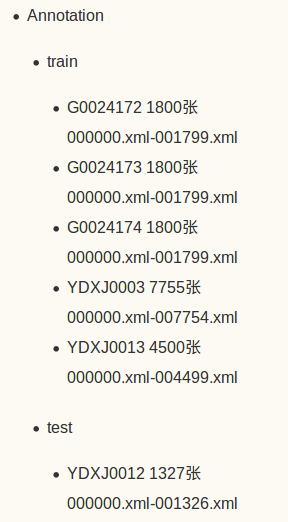
\includegraphics[width=4cm]{figures/1.png} 
	} 
	\subfigure[]{ 
		\label{p1b} %% label for second subfigure 
		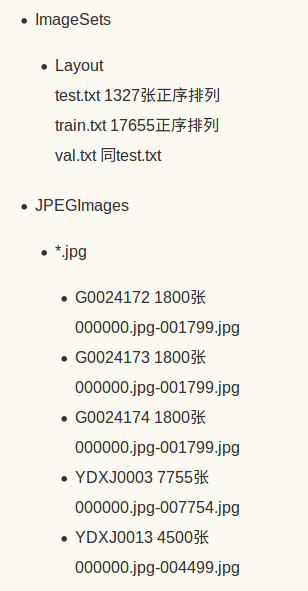
\includegraphics[width=4cm]{figures/2.png} 
	} 
	\caption{URPC2018 data sets architecture} 
	\label{p1} %% label for entire figure 
\end{figure}

\subsection{Train a Contest Model}

We put organised data sets to the remote server and try to train a model that can meet requirement of contest. Before doing like this, appropriate code modification is necessary because self.classes and label is not as same as VOC. In the project of Faster R-CNN files, relevant codes in pascal\_voc.py need to revise, for example contents in self.\_classes variable has become what we want that are seaurchin, scallop and seacucumber.

I get the first contest trained model on Wednesday after two days running code on the server. Then I run demo.py to test the performance of model by two randomly selected pictures as shown in Fig.~\ref{p2}.
\begin{figure}
	\centering 
	\subfigure[]{ 
		\label{p2a} %% label for first subfigure 
		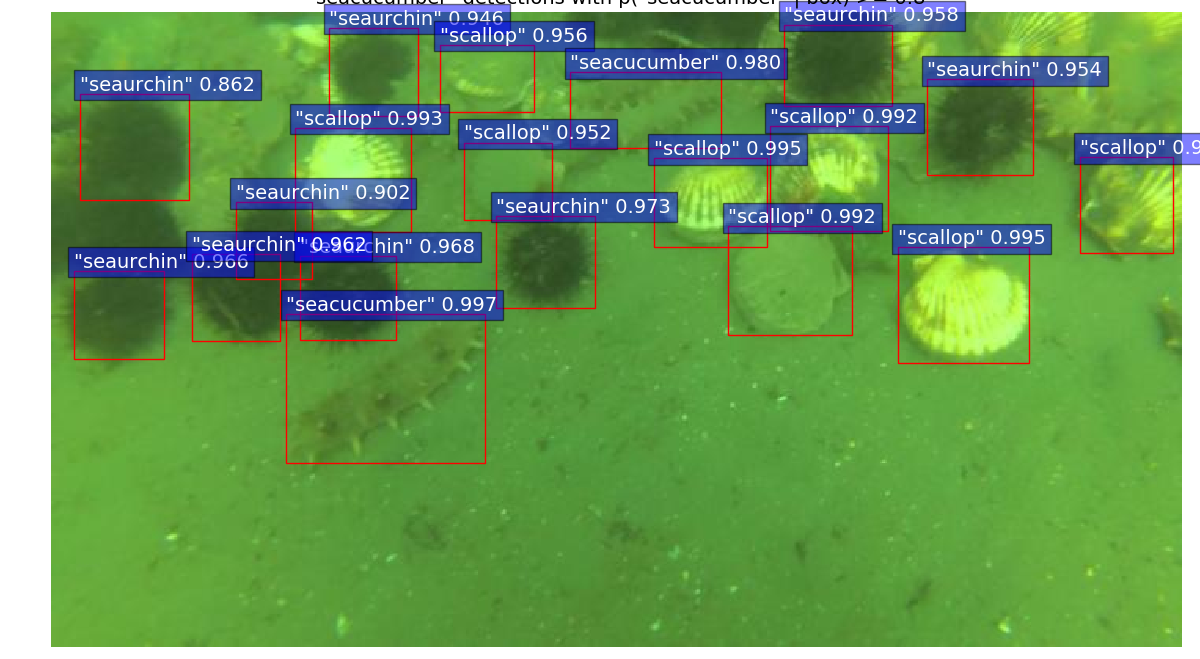
\includegraphics[width=6cm]{figures/3.png} 
	} 
	\subfigure[]{ 
		\label{p2b} %% label for second subfigure 
		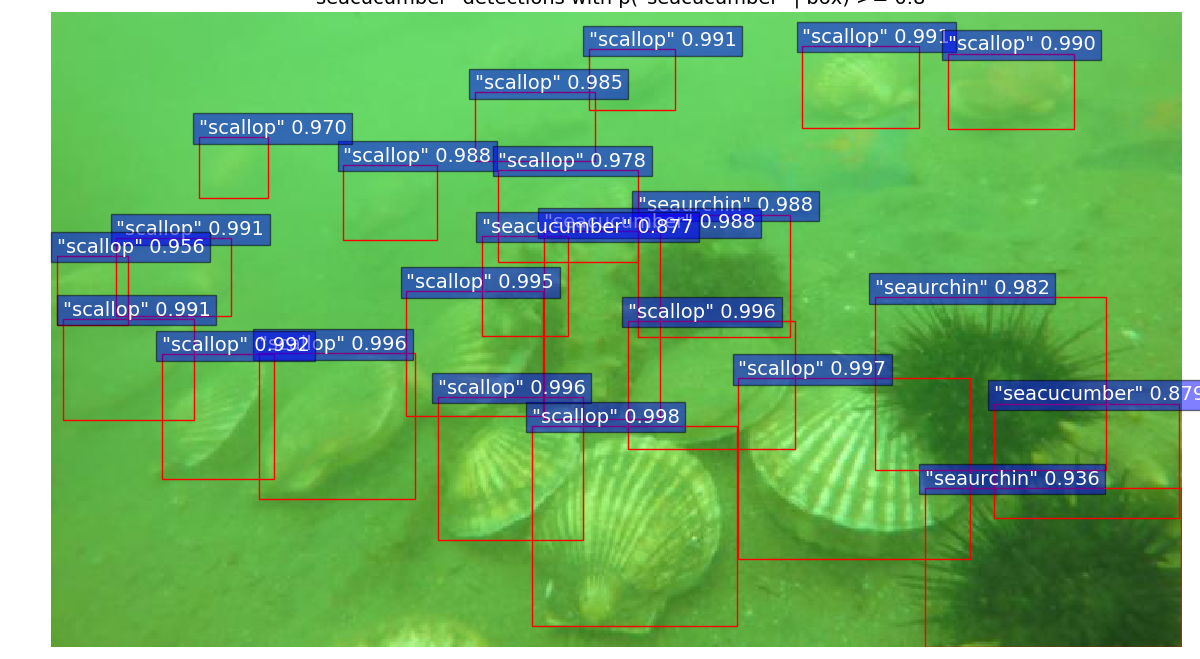
\includegraphics[width=6cm]{figures/4.png} 
	} 
	\caption{Experimental results of the first contest model.} 
	\label{p2} %% label for entire figure 
\end{figure}

Furthermore, I should check total loss of my model in Fig.~\ref{p3} to learn more about my model. Simulation results prove that this improved algorithm achieves an effect in accelerating the converging rate.
\begin{figure}
	\begin{center}
		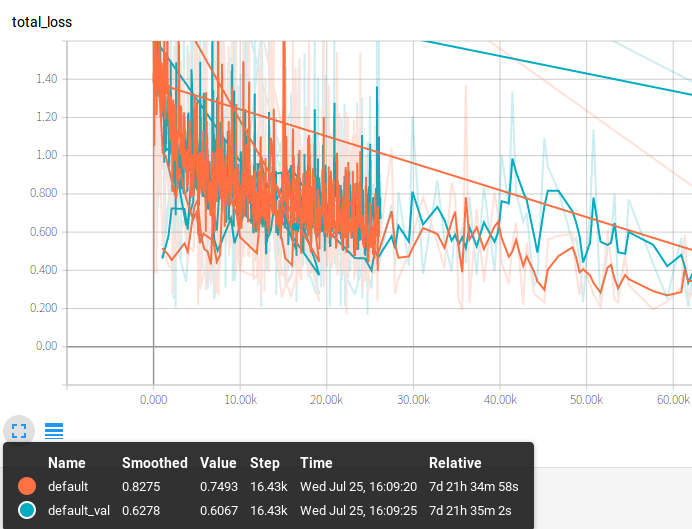
\includegraphics[scale=0.4]{figures/5.png}
	\end{center}
	\caption{Scalars in tensorboead.}
	\label{p3}
\end{figure}

\section{Plan}

\begin{tabular}{rl}
	\textbf{Objective:} & Finish training a model with contest data sets for URPC2018 \\
	\textbf{Deadline:} & 2018.07.24
\end{tabular}

\begin{description}
	\item[\normalfont 2018.07.16---2018.07.22] Finish neural networks and Deep Learning.
	\item[\normalfont 2018.07.23---2018.07.29] Finish improving deep neural networks courses.
	\item[\normalfont 2018.07.30---2018.08.05] Finish structuring machine learning projects courses.
	\item[\normalfont 2018.08.06---2018.08.12] Finish convolutional neural networks courses.
	\item[\normalfont 2018.08.13---2018.08.19] Finish sequence models courses.
\end{description}



% If you don't cite any references, please comment the following two lines
\bibliographystyle{ieee}
\bibliography{ref.bib}

\end{document}